\documentclass[11pt,a4paper]{article}
\usepackage[margin=22mm]{geometry}
\usepackage[T1]{fontenc}
\usepackage{lmodern,booktabs,amsmath,bisse-sketch}
\setlength{\parindent}{0pt}
\setlength{\parskip}{7pt}
\begin{document}
{\LARGE\sffamily\bfseries BiSSE icons: sketch-matched version}\par
The supplied geometry is preserved: touching state blocks, right-angle splits,
unnumbered circles, crosses and a no-event symbol. State 0 is light, softened orange;
state 1 is deep blue. Extinction crosses are vivid crimson. The state colors
differ in both hue and lightness; extinction also has its distinct cross shape.

\begin{center}
\renewcommand{\arraystretch}{1.3}
\begin{tabular}{@{}p{65mm}cc@{}}
\toprule
 & State 0 & State 1\\\midrule
State change ($0\to1$ / $1\to0$) & \bisseBlocks{0}{1} & \bisseBlocks{1}{0}\\[3mm]
Split, upper daughter extinct & \bisseUpper{0} & \bisseUpper{1}\\[3mm]
Split, lower daughter extinct & \bisseLower{0} & \bisseLower{1}\\[3mm]
Extinction (state-independent symbol) & \multicolumn{2}{c}{\bisseDeath}\\[3mm]
Nothing happens & \multicolumn{2}{c}{\bisseNoEvent}\\\bottomrule
\end{tabular}
\end{center}

\textbf{Legend.} Read evolution from left to right. All three circles in a split
have the same state: BiSSE speciation does not change state. The cross identifies
the daughter whose descendants eventually die out; it does not require immediate
extinction at speciation. The slash-circle means \emph{no event} in this custom
legend, not an empty clade or extinction. In equations, its probability is
$1-(\lambda_i+\mu_i+q_{ij})\Delta t$ to first order.

\subsection*{Overleaf}
Upload this project, or copy \texttt{bisse-sketch.sty} into an existing project.
\begin{verbatim}
\usepackage{bisse-sketch}  % in the preamble

\bisseBlocks{0}{1}
\bisseBlocks{1}{0}
\bisseUpper{0}   \bisseUpper{1}
\bisseLower{0}   \bisseLower{1}
\bisseDeath
\bisseNoEvent
\end{verbatim}
Set a width with, for example, \verb|\bisseUpper[18mm]{1}|.
Individual vector PDFs are in \texttt{icons/}; for example:
\begin{verbatim}
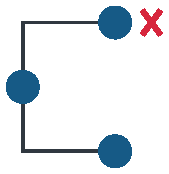
\includegraphics[width=18mm]{icons/split-upper-1.pdf}
\end{verbatim}
No numerals, gradients, shadows, grid background or red/green pairing are used.
The palette can be adjusted by redefining \texttt{bisseBlue}, \texttt{bisseOrange},
\texttt{bisseOrangeOutline}, \texttt{bisseExtinct} and \texttt{bisseDark} after loading the package.
\end{document}
